\chapter{Implementation}
\thispagestyle{main} % Needed for Footer and Header on Chapterpage
This chapter focuses on explaining why things were implemented in a certain manner. In this chapter the trade-offs and decisions which were made while building the VM are documented. Since this should be useful for follow-up work, it was done in a way that makes it easier to decide if something needs to be changed or to help reach the same conclusion.

\section{Software Architecture}
Figure \ref{package overview} shows the structure of the project on package-level and the dependencies among packages. The miner application was built with software engineering principles in mind. Particular attention was paid to modularity. This made it easy to integrate the virtual machine into the existing miner application. Furthermore, the following figure shows which packages were added and which where modified to integrate smart contracts into the Bazo Blockchain. As the miner and all other projects are written in Go, the new components are written in Go as well.
\begin{figure}[H]
	\begin{center}
	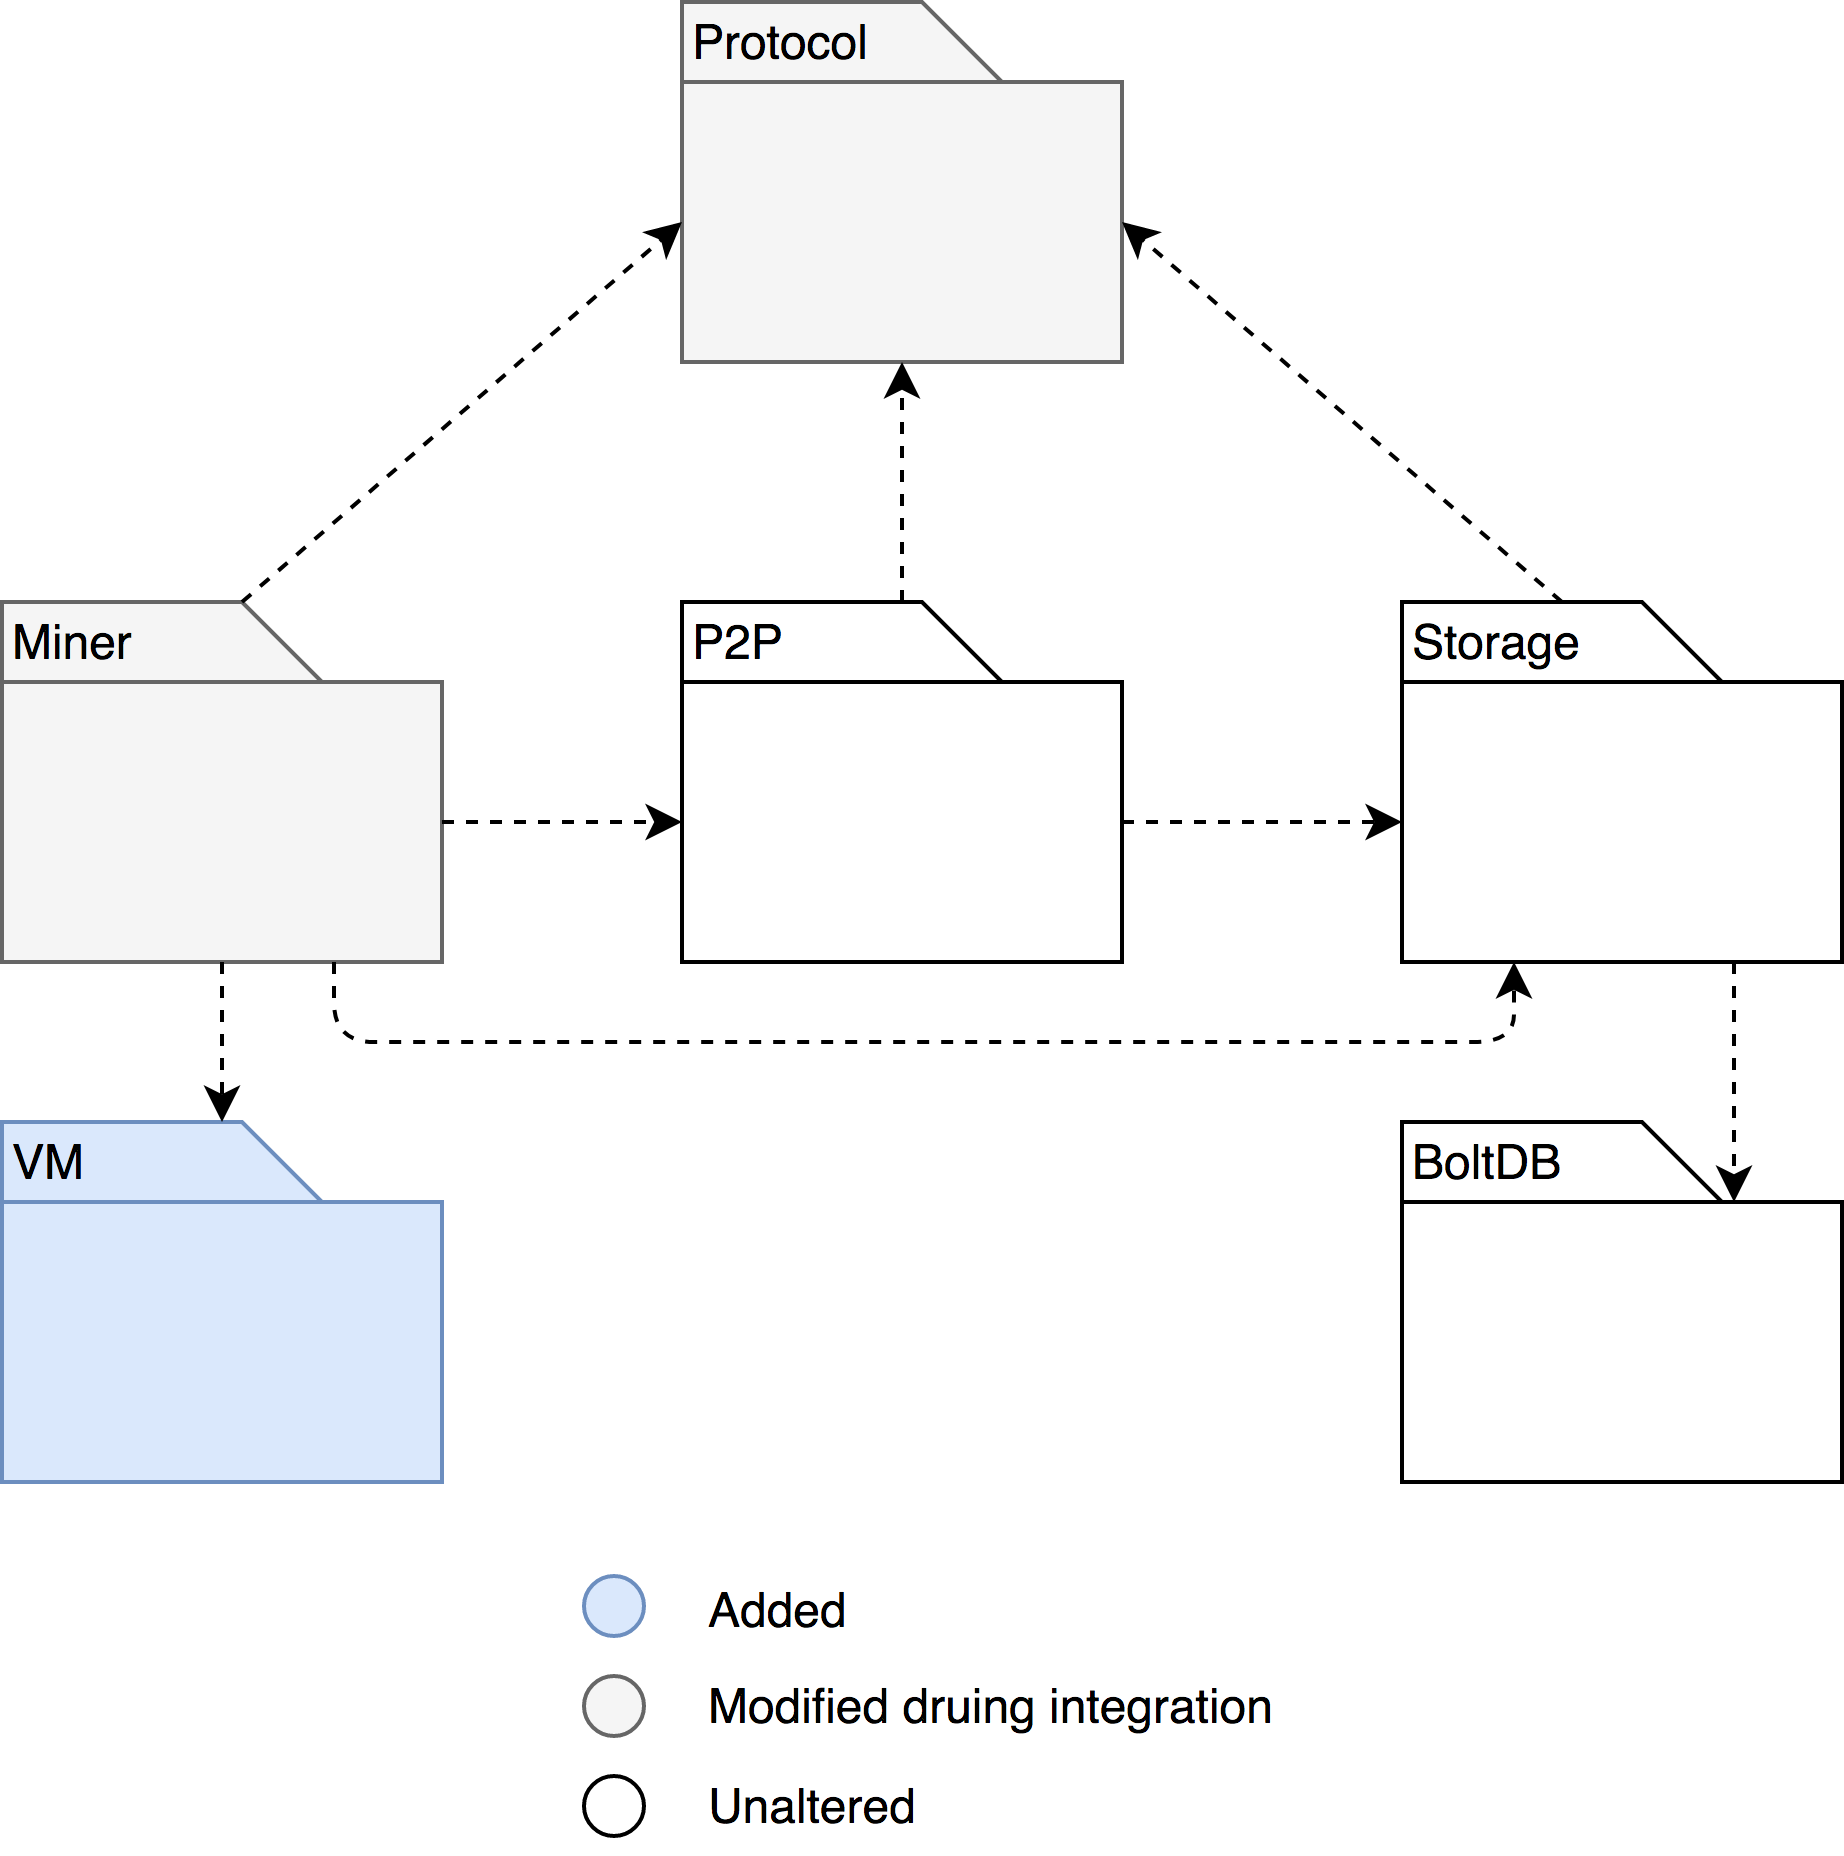
\includegraphics[width=0.8\textwidth]{./images/package-diagram}
	\caption{UML Package Diagram}
	\label{package overview}
	\end{center}
  \end{figure}

\begin{description}
	\item[Protocol] This package contains the building blocks for the Bazo Blockchain. In particular it contains the structure, encoding, decoding and hashing functions of all transaction types, blocks and accounts. In addition a transaction interface is defined, allowing an abstract treatment of transactions. \cite{ba_miner}
	\item[Miner] The miner package contains all mining related components. This includes the validation and consolidation of transactions into blocks, the calculation of the consensus mechanism and the building of the merkle tree. In addition to that, blockchain related tasks such as rollback operations and state changes are contained in this package. Access to \textit{P2P} and \textit{Storage} packages are needed in order to handle transactions over the network and signal storage-related operations. \cite{ba_miner} To execute the virtual machine and access its results, the miner also needs access to the \textit{VM} package.
	\item[VM] This package contains the virtual machine itself and all its components, namely the evaluation stack, the call stack, the implementations of data structures and all available opcodes.
	\item[P2P] All networking related operations are implemented in the \textit{P2P} package \cite{ba_miner}. Since for the integration of the virtual machine nothing had to be changed, the content of this package is not discussed any further.
	\item[Storage] The storage package is concerned with memory-related tasks. The lower-level functionality was implemented with the external \textit{BoltDB} package. Since entries are encoded before writing to storage and decoded when loaded \cite{ba_miner}, this package could be left unaltered. For that reason, this package is also not described further.
	\item[BoltDB] This package contains the \textit{BoltDB} package which is an external dependency. \texttt{BoltDB} is a simple, lightweight key/value base. \cite{ba_miner}
	\item[Parser] The \textit{Parser} package contains the parser, which consists of a Tokenize and Parse function and tokens. These components are needed to compile \flqq Enhanced Bazo Byte Code\frqq{ } to a byte code instruction set that can be interpreted by the virtual machine. This package is completely stand-alone and does not have any dependencies. The package is also kept in a separate repository.
\end{description}

\section{Protocol}
As mentioned in Chapter \ref{design_miner} the structs of Account, FundsTx and AccTx had to be adapted. The structs originally had a fixed length. The structs are transferred encoded between the individual components. The original encoding and decoding functions of those structs is based on the fixed length of the struct. Since the added fields are optional and have an arbitrary length, the encoding and decoding functions had to be redesigned. It was decided to use the gob package, which is a package from the Go standard library. The gob package manages streams of binary values between an encoder and decoder. A stream of gobs is self-describing. \cite{golang_gob} The main disadvantage is that these functions are no longer platform independent. It was decided to use gob since all other software system which directly interact with the miner are implemented in Go and because it is the fastest standard encoding library in Go. 

\subsection{Encoding}
The new encoding function for the AccTx struct is shown in figure \ref{new_encode}. Switching to gob has lead to a better readability and to fewer lines of code. The type information is defined in line 2. The function \mintinline{go}{.Encode()} in line 12 makes sure that all type information data is sent before it is needed. \cite{golang_gob} The encoding functions of the other structs, that were redesigned are very similar and therefore not further described.

\begin{figure}[thp]%
    	\centering
		\begin{minipage}{0.7\textwidth}
		\begin{minted}
		[
		frame=lines,
		autogobble,
		framesep=2mm,
		baselinestretch=1.2,
		fontsize=\footnotesize,
		linenos
		]{go}
		func (tx *AccTx) Encode() (encodedTx []byte) {
			encodeData := AccTx{
				tx.Header,
				tx.Issuer,
				tx.Fee,
				tx.PubKey,
				tx.Sig,
				tx.Contract,
				tx.ContractVariables,
			}
			buffer := new(bytes.Buffer)
			gob.NewEncoder(buffer).Encode(encodeData)
			return buffer.Bytes()
		}
		\end{minted}
		\caption{New gob based encoding function}
		\label{new_encode}
		\end{minipage}
\end{figure}

\subsection{Decoding}
Figure \ref{new_decode} shows the decoding function of AccTx. The \mintinline{go}{decoder.Decode()} function in line 5 reads the next value from the input stream and stores it in the data represented by the AccTx interface. \cite{golang_gob}

\begin{figure}[thp]%
    	\centering
		\begin{minipage}{0.7\textwidth}
		\begin{minted}
		[
		frame=lines,
		autogobble,
		framesep=2mm,
		baselinestretch=1.2,
		fontsize=\footnotesize,
		linenos
		]{go}
		func (*AccTx) Decode(encodedTx []byte) *AccTx {
			var decoded AccTx
			buffer := bytes.NewBuffer(encodedTx)
			decoder := gob.NewDecoder(buffer)
			decoder.Decode(&decoded)
			return &decoded
		}
		\end{minted}
		\caption{New gob based decoding function}
		\label{new_decode}
		\end{minipage}
\end{figure}

\section{Miner}
This section describes what changes had to be made to the miner to integrate the VM.
\subsection{Constructors}
\textit{AccTxs} now have an optional field for contracts and contract variables. If the \textit{AccTx} is meant to create an external account nil has to be passed for both parameters in the constructor. If the \textit{FundsTx} is intended to transfer coins, the data field has to be nil.

\subsection{VM Entry Point}
The balance of a FundsTx is updated in \mintinline{go}{addFundsTx()} in the block.go file. Therefore, it was decided to use it as entry point for the VM. Figure \ref{addFundsTx} shows the function without parts that are irrelevant for the integration. Before the function checks whether the transaction calls a smart contact, it performs various checks, i.e. if the account exists or if the sender has a balance high enough to transfer the defined amount of Bazo coins. If all these checks are successful the function validates if the transaction is a valid smart contract call. If so, a new context object with the receiver account and the transaction is created as seen in line 8. As next step the virtual machine is initialized with the context object. In line 12 the \mintinline{go}{Exec()} function is called which starts the virtual machine. If the \mintinline{go}{Exec()} function returns with an error the execution of the addFundsTx is aborted and the context changes are not persisted. After the VM execution, the finalizing steps are carried out, such as updating the balances of both accounts and writing the block header to storage.

\begin{figure}[thp]%
    	\centering
		\begin{minipage}{0.8\textwidth}
		\begin{minted}
		[
		frame=lines,
		autogobble,
		framesep=2mm,
		baselinestretch=1.2,
		fontsize=\footnotesize,
		linenos
		]{go}
func addFundsTx(b *protocol.Block, tx *protocol.FundsTx) error {
	... // Various checks
	// Check if transaction has data and receiver is a smart contract account
	if tx.Data != nil && b.StateCopy[tx.To].Contract != nil {
		context := protocol.NewContext(*b.StateCopy[tx.To], *tx)
		virtualMachine := vm.NewVM(context)

		// Check if vm execution run without error
		if !virtualMachine.Exec(false) {
			return errors.New(virtualMachine.GetErrorMsg())
		}
		//Update changes vm has made to the contract variables
		context.PersistChanges()
	}
	... // Finalization
}
		\end{minted}
		\caption{addFundsTx function}
		\label{addFundsTx}
		\end{minipage}
\end{figure}

% \subsection{Adjustment of Transaction Encoding}

% \subsection{Adjustment of opcodes to context and miner}

\section{Virtual Machine}
This chapter describes the most important parts of the VM implementation and the rationale behind it.

\subsection{Stack}
\begin{tabular}[t]{ p{3cm} p{12.5cm}}
\raggedright
\textbf{Maximum Stack Size} &
Facing the concern of excess memory usage of the contract on the miner, we decided to limit the stack size to 1MB which seems to be well above what the contracts will need. We neglected using the gas amount for maximum storage determination because it would be just a soft limit. \\ \\

\raggedright
\textbf{Data Structure} &
As underlying data structure of the stack, keeping in mind to keep the code of the VM as short and simple as possible and without unnecessary conversions it was decided to use a two dimensional byte array. We neglected using a simple array of bytes as data structure where elements with greater length than a byte are pushed using multiple indexes, as it is common when having no abstraction layer. We have also neglected the use of big.Int as the underlying data type which is used by Ethereum. big.Int is also arbitrarily long. The reason for this decision was that converting signed operations to unsigned operations and optimizing the elimination of leading zeros posed a problem. Still, big.Int was used for many opcodes of the Bazo VM. A multidimensional byte array was chosen to achieve simplicity, readability and extendability of the code. The downside of smaller conversions from big.Int to byte array are accepted. \\ \\

\raggedright
\textbf{Data Type} &
It was important that the data type used for the underlying data structure of stack was of arbitrary length or at least very big because of cryptographic applications. Splitting up an element into multiple bytes so that it can be saved when using an array of fixed length as underlying data structure would have been a lot more complex and more error-prone to implement. \\ \\

\raggedright
\textbf{Pass by Reference} &
We neglected working with references because even though there are more elements created on the heap of the physical machine, it shouldn't make a difference considering the vast availability of resources on modern computers and our rather small contracts. In hindsight and considering the results of Chapter \ref{evaluation} working with references and using pass by reference might have improved the performance of the VM in the benchmark test. \\ \\
\end{tabular}

\subsection{VM instruction cycle} \label{exec_cycle}
This section describes the \mintinline{go}{Exec()} function shown in figure \ref{vmexecutioncycle}. The instruction cycle can be described as an end-less loop with a switch statement that interprets the instructions one after another and acts accordingly.

\begin{tabular}[t]{ p{3cm} p{12.5cm}}
\raggedright
\textbf{Precondition} &
The virtual machine is embedded into the miner. Precondition that the VM instruction cycle is started is that the transaction must be sent to a smart contract account and the transaction data field is not empty. If these preconditions can be fulfilled, the VM instruction cycle is started by the miner. \\ \\

\raggedright
\textbf{Starting point} &
At the starting point of the execution cycle the virtual machine contains a set of instructions, has access to the execution context and the program counter set to zero. \\ \\

\textbf{Steps} &
The instruction cycle can be divided into three steps which are repeated over and over again until an invalid instruction occurs. Furthermore, the execution can be halted by an instruction or if the program counter is out of bounds. All this steps are handled in the \mintinline{go}{Exec()} function. These are the three steps:
\begin{description}
  \item[1. Fetch] The instruction the program counter points to is fetched. After it is fetched, the program counter is increased, which then points to the next element.
  \item[2. Decode] In this step the instruction is matched with pre-defined opcodes, which can be interpreted by switch statement of the \mintinline{go}{Exec()} function. Within this section of the function, the costs for the instruction are subtract.
  \item[3. Execute] The instruction is executed according to the opcode. There are opcodes for arithmetic operations, e.g. \mintinline{yaml}{ADD, MOD, SUB}, for flow operations e.g. \mintinline{yaml}{JMP, CALL, RET} which are allowed to change the program counter and therefore move back and forward in the instruction set, cryptographic operations, such as \mintinline{yaml}{SHA3, CHECKSIG} and context operations, e.g. \mintinline{yaml}{ADDRESS, ISSUER, CALLER, CALLDATA} that can be used to push context data composed from the transaction and the receiver account to the stack and opcodes for storing and loading state variables \mintinline{yaml}{SSTORE, SLOAD}. All implemented opcodes are listed in table \ref{opcode_table}.
    \end{description}
\end{tabular}

\begin{tabular}[t]{ p{3cm} p{12.5cm}}
\raggedright
\textbf{Return Value} &
The \mintinline{go}{Exec()} function returns a boolean. If the return value is true the execution was successful and no error occurred. If the return value is false an error occurred. \\ \\

\textbf{Persisting state variables} &
Changes to the state variables are loaded and persisted explicitly. That means, when loading a state variable a copy is pushed to the stack, all changes are made to the copy. The changes are only persisted if the \mintinline{go}{Exec()} function returns with true. This way, there is no need to roll back if the contract could not be executed successfully.
\end{tabular}

\subsection{Error handling}
\begin{tabular}[t]{ p{3cm} p{12.5cm}}
\raggedright
\textbf{Problem} &
Since the virtual machine just processes one instruction after another and as the contracts are currently written in the opcodes directly, it is easily possible to make a mistake and write a contract which the VM can not execute. \\ \\

\raggedright
\textbf{Example} &
An example for this is an opcode which tells the VM to push six bytes on the stack, when there is only one byte left in the instruction set. This causes an error in the VM which could terminate the miner. This should neither be possible by accident nor by choice. \\ \\

\raggedright
\textbf{Solution} &
As a result, many guards in front of operations which could panic have been placed. This allows the graceful failure of the VM. As the error handling of Go works over separate return values they have been added to the functions and if an error occurs, it is pushed on top of the VM stack. \\ \\

\raggedright
\textbf{Implementation} &
The message of this error object is later pushed on the stack of the VM after that the VM halts. Also to make the debugging less complicated, the name of the opcode in which the error occurred is prepended to the error message. Therefore, it is possible to determine what caused the error up to instruction type. An example error message is shown in Figure \ref{pushtestfailure}. \\ \\

\begin{figure}[H]
	\begin{center}
	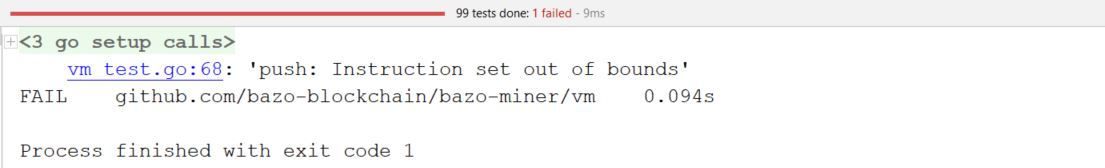
\includegraphics[width=\textwidth]{./images/push-test-failure}
	\caption{Example of an error message.}
	\label{pushtestfailure}
	\end{center}
\end{figure}

\raggedright
\textbf{Things Left Out} &
It would also have been possible to provide the number of the instruction that failed but as the code of a contract gets larger and as the instructions are not enumerated, it becomes very time consuming to count all codes to determine which one failed. This seemed not to add value or make contract creation easier and therefore this has been neglected. \\ \\
\end{tabular}

\subsection{Gas calculation}
The goal is to calculate the price based on the instruction and based on the size of the elements used by the instruction. This was solved by adding a gas price and a gas factor to every opcode. The gas price shows the base price of the instruction. The gas price is subtracted before the operation is executed. The gas factor is a multiplier. The length of any element popped from the stack is divided by 64, rounded up and multiplied by the gas factor. The result of this equation is the gas cost that is subtracted when elements are popped from the stack. This ensures that a sufficient amount of gas is available, before the actual manipulation is done. Figure \ref{gas_factor_calc} shows how the gasCost is calculated.

\begin{figure}[thp]%
    	\centering
		$
		gasCost=\left( \frac { { length }_{ element }+63 }{ 64 }  \right) \times gasFactor
		$
		\caption{Gas cost equation}
		\label{gas_factor_calc}
\end{figure}

\subsection{Trace function}
The trace function is activated by passing true as a parameter to the \mintinline{go}{Exec()} function. The trace function prints the instruction that is processed, its parameters, the contents of the evaluation stack and the memory usage to the console. This is useful for debugging. Every opcode has a list of parameter types. This list shows, which parameters are taken from the instruction set. Available parameter types are \mintinline{go}{BYTES}, \mintinline{go}{BYTE}, \mintinline{go}{ADDR} and \mintinline{go}{LABEL}. The trace function loops through the parameter types list of the current opcode and treats every opcode as specified using a switch statement. Figure \ref{traceoutput} shows an example trace output.
\begin{description}
	\item[BYTES] are variable length, the first byte that follows after the opcode in the instruction set defines how many bytes are pushed. Counting starts at zero, therefore the maximum is 256 bytes.
	\item[BYTE] reads a single byte.
	\item[ADDR] reads 32 bytes from the instruction set. This type is used to read addresses.
	\item[LABEL] reads the next two bytes and threats them as an integer. This type is mainly used for control flow opcodes.
\end{description}

\begin{figure}[thp]%
    \centering
   	\begin{minipage}{0.5\textwidth}
		\begin{minted}
		[
		frame=lines,
		autogobble,
		framesep=2mm,
		baselinestretch=1.2,
		fontsize=\footnotesize,
		linenos
		]
		{bash}
0000: push   [10] (bytes)
	Stack: [[10]]
	1 of max. 1000000 Bytes in use
...........................................
0003: push   [8] (bytes)
	Stack: [[8] [10]]
	2 of max. 1000000 Bytes in use
...........................................
0006: call   11 (label) [2] (byte)
	Stack: []
	0 of max. 1000000 Bytes in use
...........................................
0011: load   [0] (byte)
	Stack: [[0 10]]
	2 of max. 1000000 Bytes in use
...
	\end{minted}
	\end{minipage}
	\caption{Trace function output}
	\label{traceoutput}
\end{figure}

\section{Opcodes}
In this section the implementation of the opcodes, the rationale behind their implementation and the most important aspects when working with them are described.
\subsection{Arithmetic}
\label{arithmetic}
\begin{tabular}[t]{ p{3cm} p{12.5cm}}
\raggedright
\textbf{Implementation} &
Arithmetic opcodes use the arithmetic operations provided by big.Int. The two elements on top of the stack are popped, the operation is executed and the result is pushed back to the stack. \\ \\

\raggedright
\textbf{Element Size} &
It is not necessary to take care of the length of the elements, since big.Int allows for elements of arbitrary size. \\ \\

\raggedright
\textbf{Signing Byte} &
Important to note is that, these operations are always signed. Therefore when pushing a number the signing byte has to be provided in the first byte by setting it to zero or one. If this is not done, an error can occur or result in strange effects, because the first byte is used to describe the sign of the number. \\ \\

\raggedright
\textbf{Rationale for big.Int} &
Concerning the implementation of arithmetic opcodes for the VM
facing the need to provide operations for large elements it was decided to use big.Int. It was and neglected to use Int64 in order to achieve the possibility to work with numbers of at least 256 byte. The downside of adjusting the gas calculation to take the element size into account was accepted. \\
\end{tabular}

\subsection{Comparison Operators}
\begin{tabular}[t]{ p{3cm} p{12.5cm}}
\raggedright
\textbf{Implementation} &
Bit operations are the two opcodes \mintinline{go}{SHIFTR} and \mintinline{go}{SHIFTL} for shifting bits to the right and the left. Same as for the arithmetic operations, this is based on the implementation of big.int. \\ \\

\raggedright
\textbf{Unsigned} &
Important to note is that these operations are primarily thought to be used for bytes. They do not parse the leading byte in order to set the sign in big.Int. This means that when these operations are used on signed numbers the result could be that the signing byte becomes greater than zero or one and the number therefore is set into an invalid state. To avoid this the opcode has to be changed or reimplemented depending on the use case. \\ \\

\raggedright
\textbf{Rationale} &
Concerning the implementation of opcodes for bit operations facing the need to provide operations for large elements it was decided to use the operations provided by big.Int instead implementing the operations by ourselves to achieve the possibility to work with numbers bigger than 256 byte. It was also decided to make the operations unsigned because they are primarily thought of as bit operations. The downsides of having to adjust gas calculation to take element size into account is accepted. If in hindsight these operations are primarily used for numbers the implementation can be changed easily. \\ \\
\end{tabular}

\subsection{Bool Operations}
\begin{tabular}[t]{ p{3cm} p{12.5cm}}
\raggedright
\textbf{Implementation} &
To the category of bool operations belong \mintinline{go}{EQ}, \mintinline{go}{NEQ}, \mintinline{go}{LT}, \mintinline{go}{GT}, \mintinline{go}{LTE} and \mintinline{go}{GTE}. All of these opcodes use the the operations provided by big.Int and all of them work with signed numbers. Only \mintinline{go}{EQ} and \mintinline{go}{NEQ} work also with bytes. \\ \\
\raggedright
\textbf{\mintinline{go}{EQ} and \mintinline{go}{NEQ}} &
While writing the integration tests it turned out that the opcodes \mintinline{go}{EQ} and \mintinline{go}{NEQ} are oftentimes used for the comparison between function hashes in the ABI. Since function hashes are not signed numbers but just bytes it was decided to make these operations unsigned because the parsing of the signing byte would destroy the byte representation of the hash. As a result, signed numbers and bytes can be compared. \\ \\

\raggedright
\textbf{Rationale} &
As mentioned before the most prominent use case for \mintinline{go}{EQ} and \mintinline{go}{NEQ} is the comparison of function hashes. Therefore, they are unsigned. For the other opcodes an order has to exist and therefore the first byte of the elements is parsed to set the sign of the big.Ints on which the operation is performed on. \\ \\
\end{tabular}

\subsection{Control Flow Operations}
\begin{tabular}[t]{ p{3cm} p{12.5cm}}
\raggedright
\textbf{Implementation} &
Control flow opcodes like \mintinline{yaml}{JMP} are used to change the  the program counter and therefore changing the sequence of execution. These opcodes read labels from the instruction set. \\ \\

\textbf{Call Stack} &
The \mintinline{yaml}{CALL} and \mintinline{yaml}{CALLIF} opcodes are special, since a new call stack is allocated when they are executed. The call stack has a return address and copies of the values that are passed to the call stack. How many values have to be passed to the call stack is provided by an argument of the \mintinline{yaml}{CALL} and \mintinline{yaml}{CALLIF} opcode. These copies are used for the operations within the scope of the called function. \mintinline{yaml}{RET} is used at the end of the function to jump back to the return address. The remaining values on the call stack are pushed to the evaluation stack and the call stack is deleted. \\ \\

\raggedright
\textbf{Rationale} &
Control flow opcodes are essential to make the virtual machine Turing complete. Having this type of opcodes allows the contract creator to build loops and conditions. With the introduction of a call stack, the implementation of function calls was realized. \\ \\

\end{tabular}

\subsection{Data Structures}
\begin{tabular}[t]{ p{3cm} p{12.5cm}}
\raggedright
\textbf{Overview} &
The two basic data structures map and array are directly implemented as opcodes. Structs could be created on top of an array. For each data structure opcodes are available to add, remove, set and retrieve values.\\ \\

\raggedright
\textbf{Implementation} &
Both data structures were implemented on top of a byte array. 
The required methods to add, remove, set and retrieve values for both data types have been implemented.
 \\ \\

\raggedright
\textbf{Rationale} &
The ability to marshal the data structures into a byte array in order to push it on the stack was important. The overhead for doing this should be as low as possible. Further important concerns are keeping the implementation simple and the contents of the structure viewable in the trace function for debugging. It was decided to implement the data structures on top of byte array. The possibility of using the Go native implementation of map and array were neglected. The reasons for this decision are that the array or map would have to be marshalled and unmarshalled by each opcode in order to pop the data structure from the stack, perform the operation and push it back. Also, an array of bytes could not be used as an index for a map since it is not comparable. The heightened possibility of errors in the implementation is accepted since the blockchain is a research blockchain although measures have been taken to provide as much correctness as possible.  \\ \\
\end{tabular}
\section{Context}
For the VM execution to have any effect it is necessary to change the miner's state eventually. This section describes how the state changes of a contract execution are persisted and explains the data the context is composed with. Furthermore, Figure \ref{context_interface} shows the interface for the VM context.

\begin{tabular}[t]{ p{3cm} p{12.5cm}}
\raggedright
\textbf{Consistency} &
One problem with an immediate change of the miner's state is that the contract execution could fail in the middle of the contract resulting in inconsistencies. Such inconsistencies could be resolved with a rollback but this was neglected since this is more complicated to implement than letting the VM work on copies. Therefore, it was decided to provide the VM with copies of the state variables. \\ \\

\raggedright
\textbf{Decoupling} &
In order to reduce the coupling of the miner it was decided to provide the access to the state variables via a context object which implements the necessary getters and setters. The context object contains the logic needed to create copies and to avoid encapsulation breaches. The context object is setup by the miner, the reference to it is then passed to the VM and the changes are written back after a successful execution of the contract by the miner again. \\ \\

\raggedright
\textbf{Readability} &
To clearly describe which operations the VM uses to access state variables in the code of the VM an interface was created which the VM uses and the context implements. If necessary this would also allow for easier testing since this makes the mocking and overwriting of specific methods of the context possible. \\ \\
\end{tabular}

\begin{figure}[thp]%
    \centering
    \begin{minipage}{0.8\textwidth}
	\begin{minted}
		[
		frame=lines,
		autogobble,
		framesep=2mm,
		baselinestretch=1.2,
		fontsize=\footnotesize,
		linenos
		]
		{go}
		type Context interface {
			GetContract() []byte
			GetContractVariable(index int) ([]byte, error)
			SetContractVariable(index int, value []byte) error
			GetAddress() [64]byte
			GetIssuer() [32]byte
			GetBalance() uint64
			GetSender() [32]byte
			GetAmount() uint64
			GetTransactionData() []byte
			GetFee() uint64
			GetSig1() [64]byte
		}
	\end{minted}
	\end{minipage}
	\caption{Context interface}
	\label{context_interface}
\end{figure}


\subsection{Data from a Transaction}
\begin{description}
  \item[Sender/Address] The sender field shows the public address of the transaction sender 
  \item[Fee] The maximum price the transaction can cost.
  \item[TransactionData] This field contains the identifier to the function the sender wants to call on a certain smart contract and its arguments. In order to identify the function and still being able to override functions and enable polymorphism, the identifier is a hash build from the function signature (name and parameters).
  \item[Amount] This field shows the amount of Bazo units send in this transaction.
\end{description}

\subsection{Data from the Receiver Account}
\begin{description}
  \item[Issuer/Owner] This field contains the public address of the account owner.
  \item[Balance] This field contains the number of coins in this account.
  \item[Contract] This field is the smart contract itself and contains the byte code. The data type is \mintinline{yaml}{[]byte}, so it can easily be packed into a transaction field.
  \item[ContractVariables] This field contains the state variables that are changed by executing transactions.
\end{description}

\section{Parser}
The language that the parser processes cannot be described as a high-level programming language and is very strongly aligned to the actual byte code. The parser package contains two classes and a test file. One class is tokens.go, which contains the available opcodes with its arguments and the token types. The second class is parser.go, which can be split into two main functions.

\subsection{Tokens class}
\begin{tabular}[t]{ p{3cm} p{12.5cm}}
\raggedright
\textbf{Token struct and types} &
Code snippet \ref{tokenstruct} shows the Token struct. The tokenType field can be \mintinline{go}{OPCODE} (Value: 0), \mintinline{go}{BYTES} (Value: 1), \mintinline{go}{BYTE} (Value: 2), \mintinline{go}{ADDR} (Value: 3), \mintinline{go}{LABEL} (Value: 4) which are all int constants. The value field contains the argument passed to the token. \\ \\
\end{tabular}

\begin{figure}[thp]%
    \centering
   	\begin{minipage}{0.4\textwidth}
		\begin{minted}
		[
		frame=lines,
		autogobble,
		framesep=2mm,
		baselinestretch=1.2,
		fontsize=\footnotesize,
		linenos
		]
		{go}
		type Token struct {
			tokenType int
			value     string
		}
		\end{minted}
	\end{minipage}
	\caption{Token Struct}
	\label{tokenstruct}
\end{figure}

\begin{tabular}[t]{ p{3cm} p{12.5cm}}
\raggedright
\textbf{Opcodes} &
The opcodes are needed to replace the opcode token with the matching value and to make sure only valid opcodes are passed. The opcodes need to be the same as in the virtual machine and also are int constants. \\ \\
\textbf{Map of opcodes} &
The map of opcodes shows which opcodes have arguments and how many arguments they have, in order to check if only the allowed amount of words is found in a single line of the contract. If more arguments than defined are passed to an opcode token, it comes to an illegal word in line exception.
 \\ \\

\end{tabular}

\subsection{Parser class}
\begin{tabular}[t]{ p{3cm} p{12.5cm}}
\raggedright
\textbf{Tokenize() function} &
The function that is run first is the \mintinline{go}{Tokenize()} function. The process of the \mintinline{go}{Tokenize()} function is shown in figure \ref{tokenizefunc}. The source code of the contract written in \flqq Enhanced Bazo Byte Code\frqq{} is passed as a string. The string is converted to a slice of lines. The \mintinline{go}{Tokenize()} function takes every first word in every line and matches it with available token types. Every first word in line must either be a comment, a label, empty or an opcode. The rest of the words in the same line are the parameters of the opcode or an inline comment, marked with a \#. Comments and empty lines are ignored. Labels end with an colon (e.g. addNums:). If the first word is a label it is added to the labelMap, to later replace it with the address.
\end{tabular}

\begin{figure}[H]
	\begin{center}
	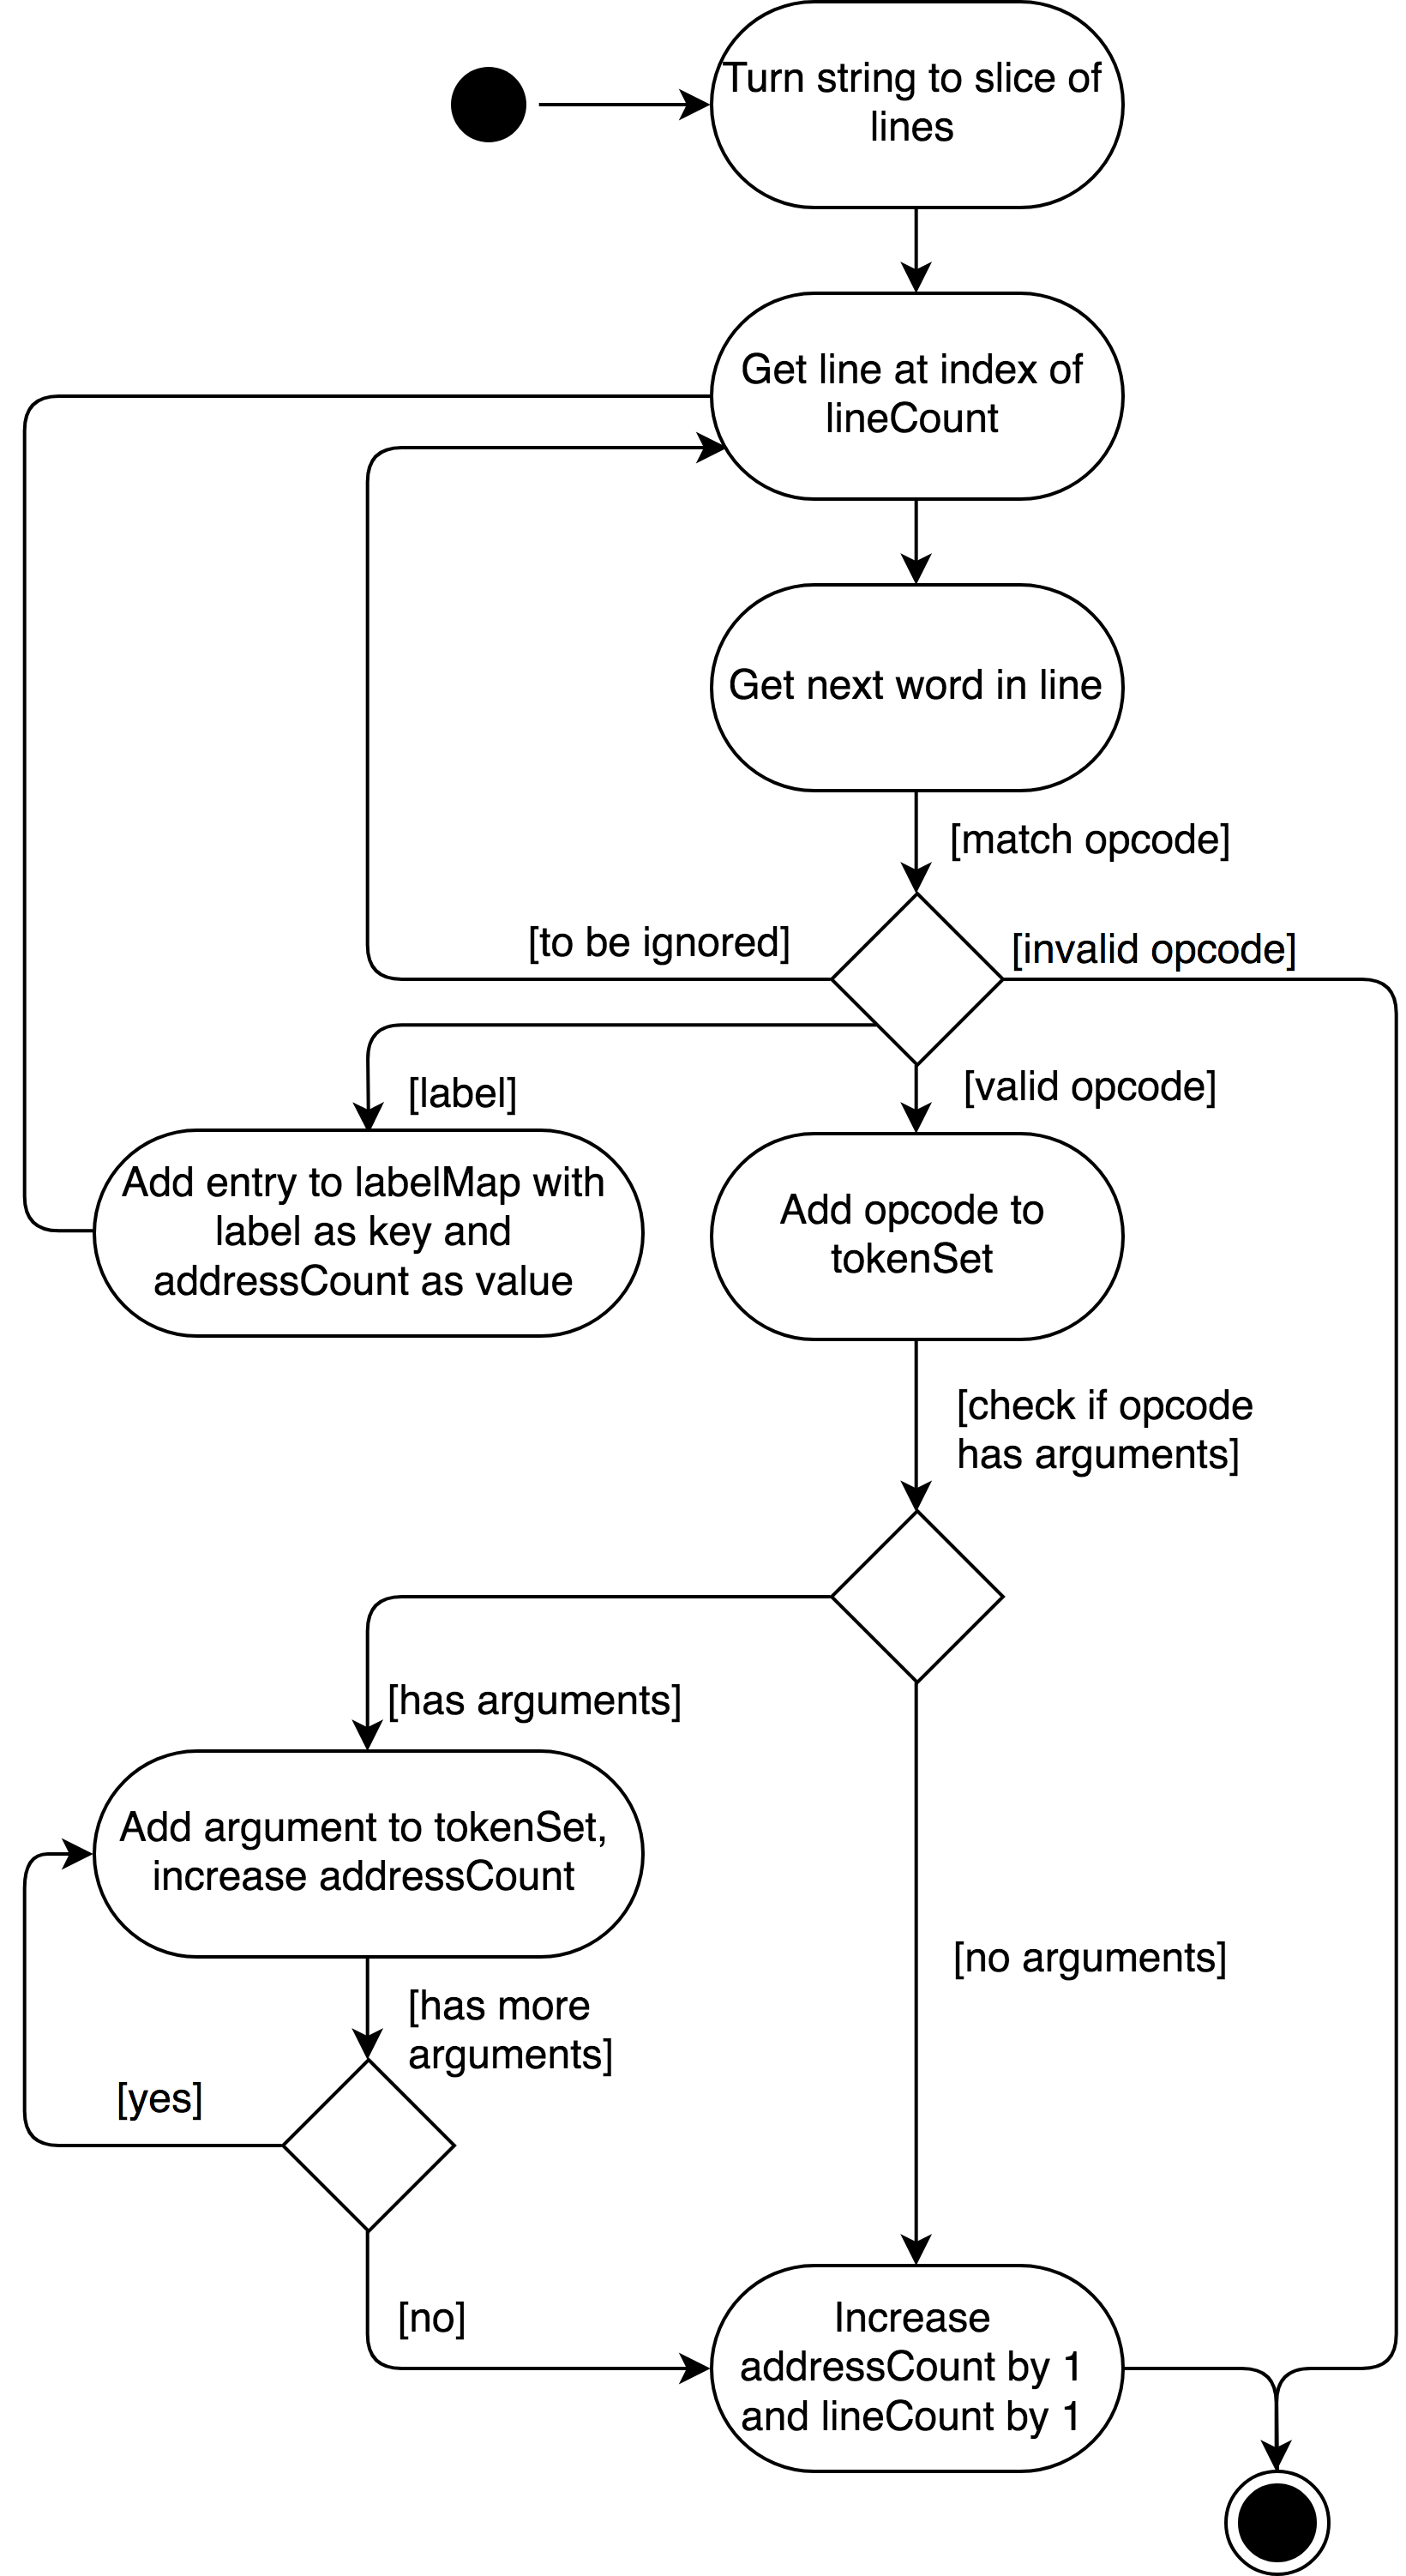
\includegraphics[width=0.5\textwidth]{./images/tokenize-function}
	\caption{UML Activity Diagram of the Tokenize Function}
	\label{tokenizefunc}
	\end{center}
\end{figure}

\begin{tabular}[t]{ p{3cm} p{12.5cm}}
\raggedright
\textbf{Token set} &
Code snippet \ref{tokenset} shows the generated token set to the basic contract shown in figure \ref{basiccontract_design} in the design chapter.
\end{tabular}

\begin{figure}[thp]%
    \centering
   	\begin{minipage}{0.4\textwidth}
\begin{minted}
[
	frame=lines,
	framesep=2mm,
	baselinestretch=1.2,
	fontsize=\footnotesize,
	linenos
]
{go}
{
[{0 PUSH} {1 55780}],
[{0 PUSH} {1 5}],
[{0 CALL} {4 addNums} {2 2}],
[{0 HALT}],
[{0 LOAD} {2 0}],
[{0 LOAD} {2 1}],
[{0 ADD}],
[{0 RET}],
}
\end{minted}
\end{minipage}
\caption{TokenSet of basic contract shown in \ref{basiccontract_design}}
\label{tokenset}
\end{figure}

\begin{tabular}[t]{ p{3cm} p{12.5cm}}
\raggedright
\textbf{Parse() function} &
The \mintinline{go}{Parse()} function compiles the token set to \flqq Bazo Byte Code\frqq. Figure \ref{parsefunc} shows the process of the function. The function iterates over all tokens in the token set and matches the different types. If the type is \mintinline{go}{OPCODE} the matching byte value is added to the instruction set. If the type is \mintinline{go}{LABEL} the value is loaded from the labelMap, which is the jump address. A special type is \mintinline{go}{BYTES}. If an opcode takes \mintinline{go}{BYTES} as an argument the first byte of the value shows the length of the byte representation. That means, that the byte representation of the value must be prepended with the amount of bytes. \mintinline{go}{BYTE} and  appends a single byte value to the instruction set. \mintinline{go}{ADDR} appends 32 bytes to the instruction set.
\end{tabular}

\begin{figure}[H]
	\begin{center}
	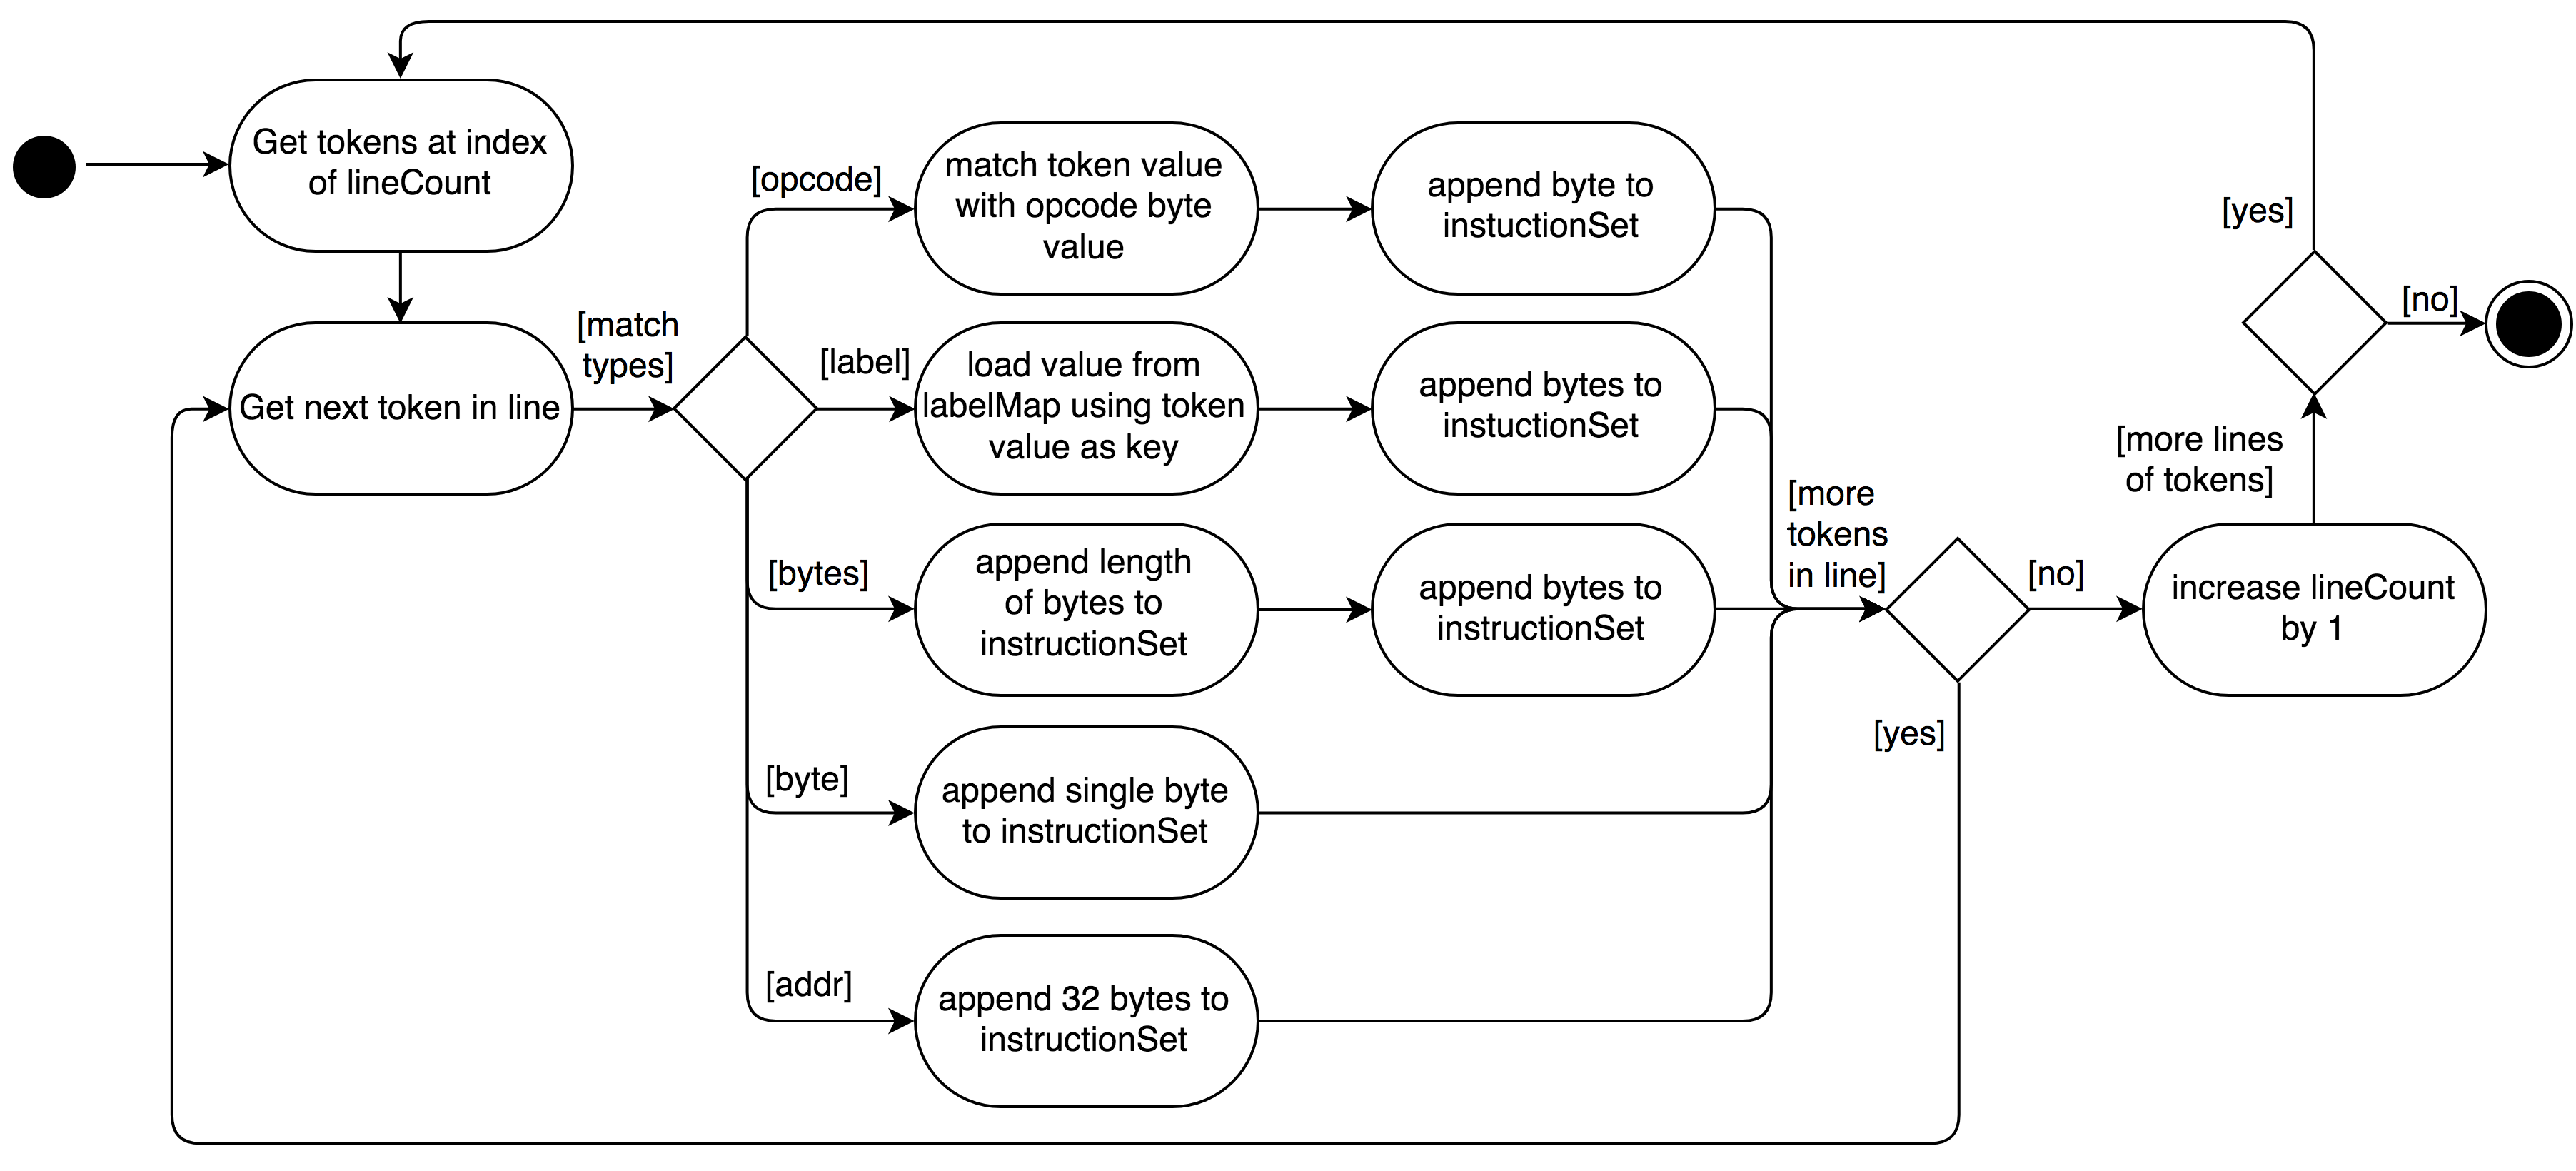
\includegraphics[width=\textwidth]{./images/parse-function}
	\caption{UML Activity Diagram of the Parse Function}
	\label{parsefunc}
	\end{center}
\end{figure}

\begin{tabular}[t]{ p{3cm} p{12.5cm}}
\raggedright
\textbf{Instruction set} &
Code snipped \ref{compiledbytecode} shows the resulting byte code instruction set.
\end{tabular}

\begin{figure}[thp]%
    \centering
   	\begin{minipage}{0.7\textwidth}
\begin{minted}
[
	frame=lines,
	framesep=2mm,
	baselinestretch=1.2,
	fontsize=\footnotesize,
	linenos
]
{go}
{
  0, 1, 217, 228, 0, 0, 5, 21, 0, 13, 2, 50, 28, 0, 28, 1, 4, 24,
}
\end{minted}
\end{minipage}
\caption{Basic contract compiled to \flqq Bazo Byte Code\frqq}
\label{compiledbytecode}
\end{figure}

\section{Testing}
The virtual machine, the parser and integration were extensively tested from the start. Depending on the type of component and its relations, different testing methods have been applied. Overall a relatively high test coverage could be achieved. In the sections below, the different testing methods for each package are explained.

\subsection{Unit Testing}
All packages have been unit tested. Each modified package is compared with the package before integration to ensure that the test coverage is not negatively affected by the integration.

\begin{tabular}[t]{ p{3cm} p{12.5cm}}
\raggedright
\textbf{Protocol} &
As described in the sections before, not many changes have been made to the Protocol package. The test coverage before the VM integration was 70\%. The updated test coverage is 68\%. The reason for a lower coverage is that the vm\_context.go class has been added, which has many getters and setters that do not need to be tested. \\ \\
\textbf{Miner} &
The test coverage before the VM integration was 65\%. The updated test coverage is 65\%, which shows that the integration has not negatively affected the coverage. \\ \\
\textbf{VM} &
The overall statement coverage is 81\%. Every component of the vm package has a test coverage over 79\%. The main component is the vm.go class. For every opcode at least one unit test has been made. Arithmetic opcodes are based on the big.Int implementation, which has been considered tested. This test coverage is influenced by the fuzz test described in Section \ref{fuzz_testing}. \\ \\
\textbf{Parser} &
The parser should be seen as a utility that is not part of the core project. For this reason, the necessity to test of this package was of low priority. Still a test coverage of 82\% could be achieved, because the package is small and the core class consists only of two main functions and a few helper methods. \\ \\
\end{tabular}

\subsection{Fuzz Testing} \label{fuzz_testing}
An instruction set of a smart contract must never be able to crash the miner. Calling a smart contract function with malicious instructions would cause the whole blockchain to collapse. To check if the VM fails gracefully, a fuzz test was implemented which creates contracts with real random bytes and then executes them. Contracts causing the miner to crash were reproduced as unit test in order to find the bug. Once the bug was found it was mitigated. This process was repeated over and over again. Starting the fuzz test with five million random contracts with every commit to the remote repository using Travis CI and having run it with a billion random contracts over night makes us confident that every bug that could crash the miner was found and mitigated.

\subsection{Integration Testing}
To test whether the virtual machine could be successfully integrated, an integration test was made. The goal of this test is to show that deploying and calling smart contracts over transactions are possible. The integration test consists of multiple small unit tests. It was tested whether it is possible to create smart contract accounts, call functions of these smart contracts and whether state variables are persisted over several transactions.
%insert number of testcoverage
